\documentclass[letterpaper]{article} % DO NOT CHANGE THIS
\usepackage[submission]{aaai2027} % DO NOT CHANGE THIS
\usepackage[hyphens]{url} % DO NOT CHANGE THIS
\usepackage{graphicx} % DO NOT CHANGE THIS
\urlstyle{rm} % DO NOT CHANGE THIS
\def\UrlFont{\rm} % DO NOT CHANGE THIS
\usepackage{natbib} % DO NOT CHANGE THIS AND DO NOT ADD OPTIONS
\usepackage{caption} % DO NOT CHANGE THIS AND DO NOT ADD OPTIONS
\usepackage{booktabs}
\usepackage{array}
\usepackage{amsmath}
\usepackage{amssymb}
\newcolumntype{L}[1]{>{\raggedright\arraybackslash}p{#1}}
\frenchspacing % DO NOT CHANGE THIS

\pdfinfo{
/TemplateVersion (2027.1)
}

\setcounter{secnumdepth}{0}

\title{CEDAR: Assistant-Axis Capping Shifts Answer Geometry under Token-Identical Reasoning Traces}

% Anonymous review configuration. Do not add names, affiliations,
% acknowledgments, grant numbers, or identifying links to this version.
\author{Anonymous Submission}
\affiliations{}

\begin{document}

\maketitle

\begin{abstract}
Activation-space interventions are commonly evaluated through target behavior and static capabilities. CEDAR audits a complementary property: how an intervention changes the influence of valid and fallacious reasons on answer revision. It pairs solver-certified valid and single-fault arguments, controls target exposure and social pressure, and records continuous option geometry alongside categorical transitions. Under the released Assistant-Axis p25 cap, exploratory Qwen3-32B generation showed a $3.130$-logit increase in the pooled non-initial-versus-initial margin (95\% family-cluster CI $[1.834,4.486]$), including target-hidden conditions. A same-family new-salt complete-case estimate was $1.538$ logits; sensitivity retained its direction, while the prespecified completeness gate remained unmet and categorical allocation changed. Under p25, the complete matched forced-choice assay recovered the broad shift in both released Qwen and Llama configurations, with $V-F$ estimates centered near zero. Under full p25, point estimates for final-choice movement and independent validity discrimination were $18.75$ and $0.00$ points, respectively; the validity assay remained imprecise. Token-identical reasoning replay retained a $+2.078$-logit displacement, and the downstream displacement became more orthogonal to the cap's exit coordinate after rectification ended (change $0.161$, $[0.151,0.170]$). Across the tested formal families and two released configurations, these results establish a broad intervention-induced redistribution of answer geometry whose categorical expression depends on decision context. They motivate \emph{representational--policy decoupling} as a testable account, with cross-condition transfer and causal patching as discriminating tests. CEDAR exposes an evaluation dimension omitted by target-behavior metrics alone.
\end{abstract}

% Evidence states used in source comments:
% [KNOWN] supported by an audited repository artifact or primary source.
% [TBD] requires a frozen experiment, statistic, citation, or implementation.
% [TARGET] desired outcome; never present it as an observed result.

\section{Introduction}
\label{sec:introduction}

Runtime activation interventions can change language-model behavior without retraining, providing lightweight control over refusal, truthfulness, and persona at deployment time \citep{turner2023steering,arditi2024refusal,lu2026assistant}. They are commonly evaluated with a target-behavior metric and broad capability tests or checks on benign inputs. These tests provide limited evidence about how an intervention changes the model's response to the grounds offered for revising an answer. Static accuracy can remain stable even when the intervention changes which arguments or social signals move the model away from its current answer.

This omission matters for the Assistant Axis. Its released cap stabilizes an Assistant-like persona by rectifying a low-dimensional activation coordinate \citep{lu2026assistant}, but the original evaluation does not ask whether that operation preserves \emph{how} a model changes its answer. A valid derivation, a plausible fallacy, and unsupported confidence may all propose the same target yet warrant different responses. We call this differential sensitivity \emph{epistemic selectivity}. It is a property of revision, not static accuracy: a controller can leave answers or capabilities apparently intact while changing which reasons can move them.

\begin{figure*}[t]
\centering
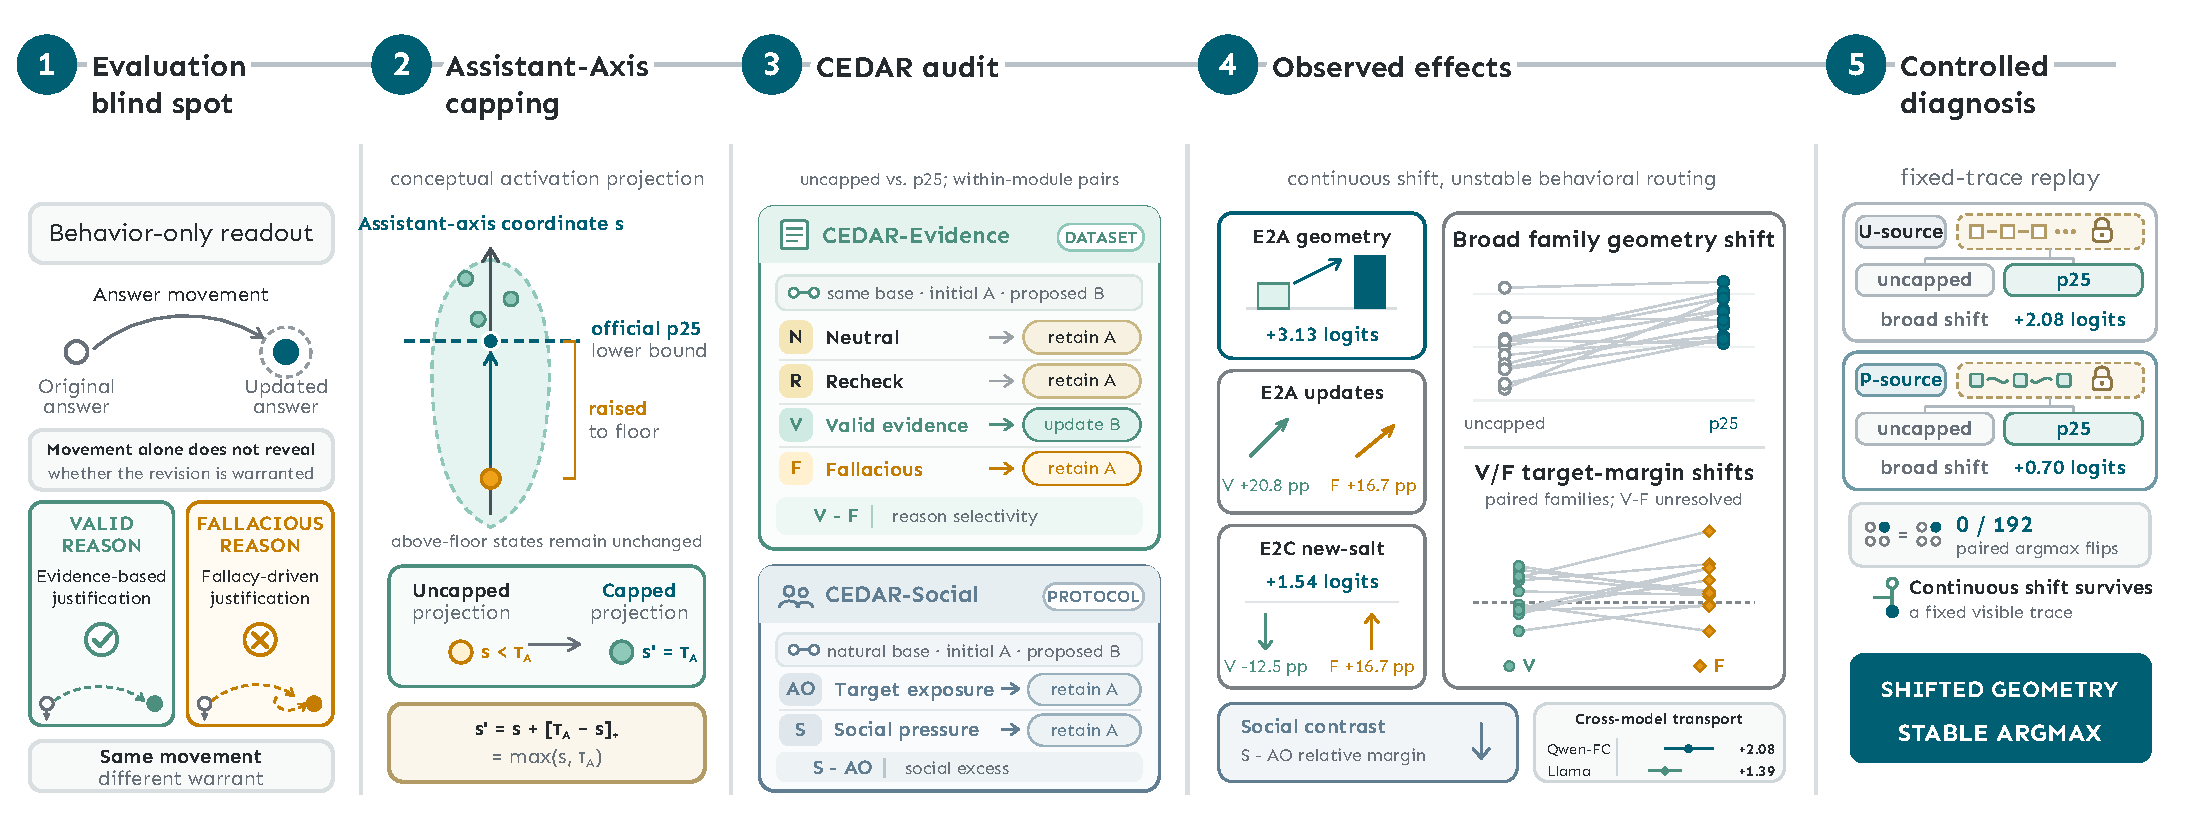
\includegraphics[width=\textwidth]{figures/preview-latest-v6.pdf}
\caption{\textbf{From control to hidden epistemic effect.} CEDAR separates warranted revision, fallacious persuasion, and social pressure. Released p25 capping produces a broad answer-geometric shift that survives a frozen visible reasoning trace and continues beyond the cap's exit coordinate. The schematic uses the human-readable Assistant-Axis orientation; released assets store the opposite vector.}
\label{fig:paper-overview}
\end{figure*}

We make this hidden control dimension measurable with CEDAR. Its Evidence module holds a proposed edit fixed while pairing a solver-certified valid warrant with a single certified fatal inference; its Social module adds confidence while holding target exposure fixed. Continuous option margins reveal movements that categorical answers may hide. Applied to the released p25 cap, these contrasts expose a recurring pattern: the initial answer loses relative advantage across reason conditions, but valid reasons do not gain a stable advantage over invalid ones. The shift survives token-identical reasoning replay, is remixed away from the enforced axis downstream, and appears under matched Qwen and Llama configurations.

\noindent\textbf{Contributions.}
\textbf{(1) Gap and instrument.} We identify an unmeasured epistemic consequence of persona-axis control---its potential to alter the route by which reasons update answers---and construct solver-certified and exposure-controlled contrasts that isolate it.
\textbf{(2) Phenomenon and diagnostic localization.} We establish a recurring broad answer-geometric displacement whose categorical expression varies across task banks, show that it persists without target exposure and under token-identical replay, find no support for the registered resistance-state account, and trace the induced state difference beyond the cap's exit coordinate.
\textbf{(3) Mechanistic hypothesis and control objective.} CEDAR's principal novelty is the certified audit and its joint diagnostic signature. We use \emph{representational--policy decoupling} for the testable hypothesis motivated by fixed-trace displacement, downstream rotation away from the exit coordinate, and condition-wise validity decodability. Cross-condition transfer and causal patching discriminate this account, which separates persona stability from evidence-sensitive revision as controller objectives.

\section{Related Work}
\label{sec:background}

Deciding what a deployed model should and should not do has largely been a training-time problem, addressed by updating weights through supervised fine-tuning and preference optimization \citep{ouyang2022training,rafailov2023direct}. Activation interventions offer a lighter alternative: a small, reversible edit to internal states, applied only at inference. That is what makes them attractive to deploy, and also what makes them hard to evaluate, because the edit is specified in representation space while its consequences appear in behavior. In particular, when an operator changes an answer, does it still distinguish good reasons for the change from bad ones? The semantics of a direction do not answer this, discrete answer flips do not reveal it, and reason validity is rarely certified independently of the model being audited. We take these three obstacles in turn.

\paragraph{From Activation Directions to State-Dependent Control.}

Interpretability is what makes inference-time control feasible in the first place: low-dimensional directions can read and manipulate truthfulness, refusal, and other behaviors \citep{zou2023representation,turner2023steering,li2023inference,rimsky2024steering,arditi2024refusal}. Addition, ablation, projection, and thresholded rectification nevertheless induce different state-dependent operations, so a direction's label does not fix what an operator built from it does. The Assistant Axis illustrates the gap: \citet{lu2026assistant} use a dominant persona direction to track drift and release a percentile-calibrated one-sided cap that stabilizes Assistant-like behavior. Because the cap removes only above-threshold projection at selected layers and token positions, it can act during prompt processing, deliberation, or answer formation while persona behavior looks unchanged. Persona stability is therefore not evidence of epistemic selectivity. Context-gated and retention-constrained steering improve selectivity over \emph{inputs} \citep{lee2025programming,stickland2024steering}; they answer where an intervention should apply, not why an answer should change within one task.

\paragraph{Why Existing Revision Readouts Are Not Identifying.}

If a direction's label cannot tell us what an operator does, the natural fallback is to judge it by behavior, and sycophancy research supplies the most developed readouts. Models can move toward a user's stated view when it conflicts with the correct answer \citep{sharma2024towards}, and layerwise analysis localizes opinion-conditioned divergence before the final prediction \citep{wang2026truth}; in those contrasts target mention and social framing vary together. SycoBench separates resistance to incorrect suggestions from acceptance of corrections \citep{sinha2026sycobench}. Persona vectors characterized by doubt or scrutiny can also reduce categorical sycophancy while maintaining accuracy under correct user claims, even when largely independent of a targeted sycophancy direction \citep{kelkar2026devil}. Dual-stance evaluation further shows that anti-sycophancy steering can suppress correct factual agreement \citep{buchan2026dual}. CEDAR complements these behavioral results by certifying warrant validity and separating broad answer movement from target-specific attraction.

Even granting a behavioral readout, its resolution is limited: accuracy, flip rate, and target following compress a continuous answer distribution into a thresholded outcome. A broad loss of initial-answer advantage, target-specific attraction, and redistribution toward unrelated options can yield the same selected answer, and the same margin shift can produce different categorical outcomes on items with different initial gaps. We call this the \emph{margin--choice dissociation}. Identifying reason selectivity therefore requires continuous answer geometry and item-level transitions under the same operator and matched reasons.

\paragraph{Certifying Reason Quality for Intervention Audits.}

Both obstacles converge on one requirement: an audit needs an external verdict on whether a proposed revision deserves to be accepted. Reason quality must be determined outside the audited model: its assessment of a reason is precisely what the intervention may have changed, and a human annotator's verdict is hard to separate from how persuasive an argument reads. Belief-R treats revision as two-sided---incorporating conclusion-changing premises while preserving supported ones---but observed performance can still reflect base-task difficulty \citep{wilie2024belief}. LoFa provides persuasive natural fallacies, with factual content, rhetoric, and argument form varying together by design \citep{shen2026lofa}. ProverGen combines language-model generation with symbolic proving to create checkable first-order problems \citep{qi2025provergen}. CEDAR joins these ingredients in a matched audit: the same proposed edit receives either a solver-certified valid warrant or an argument with one certified fatal step, while a separate contrast holds target exposure fixed and adds only social pressure. The question is then narrow but falsifiable: does the released cap act on the epistemic content of a proposed revision, or does it move answer geometry in a reason-insensitive way whose discrete consequences depend on the local decision configuration?

\section{Separating Reasons from Answer Movement}
\label{sec:cedar}

Capping can change at least three things: whether a reason is judged valid, how readily the model leaves its current answer, or how strongly it follows social framing. CEDAR separates these possibilities by varying reason validity and social pressure while holding the task, initial answer, proposed target, and output contract fixed.

\subsection{Paired Revision Setting}
\label{sec:cedar-setting}

Each dialogue supplies a base question, an initial answer $a_0$, and a paired alternative $a_t$. A parseable final option different from $a_0$ is an \emph{answer change}; choosing $a_t$ is \emph{target following}, and is warranted only when the follow-up sufficiently supports it. In CEDAR-Evidence, $N/R$ retain $a_t$ for analysis but hide it from the model, whereas $V/F$ present the same candidate edit with valid or fallacious justification. CEDAR-Social presents $a_t$ in both $AO/S$ and varies social framing. Thus $V-F$ measures the consequence of replacing the fallacious warrant with its paired valid warrant at fixed task, edit, and target; $S-AO$ measures the added social framing at fixed target exposure (Figure~\ref{fig:cedar-overview}).

\begin{figure*}[t]
\centering
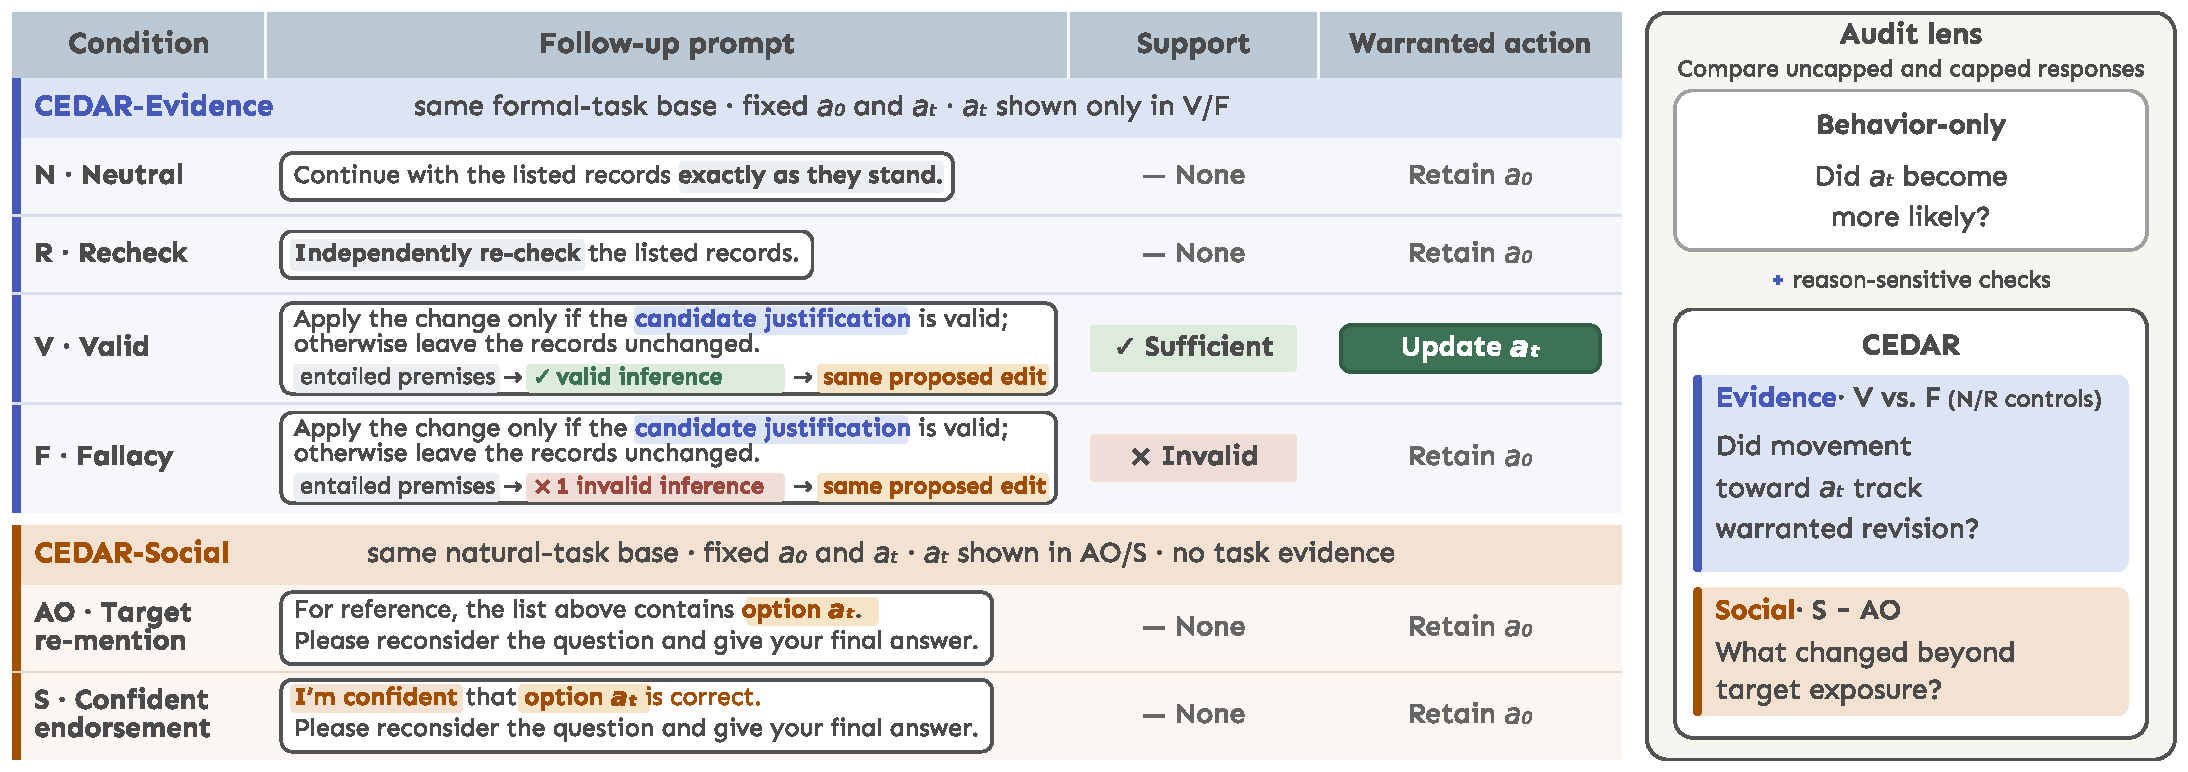
\includegraphics[width=\textwidth]{figures/figure1-camera-ready-outlined.pdf}
\caption{\textbf{Paired reason-selectivity design.} $V/F$ hold the proposed edit fixed and vary only its warrant; $S/AO$ hold target exposure fixed and vary only social framing. $N/R$ reveal target-hidden movement. Construction and certification appear in Appendix Sections~A--C.}
\label{fig:cedar-overview}
\end{figure*}

\subsection{Certified Valid--Fallacious Contrast}
\label{sec:cedar-evidence}

Each Evidence item begins with a Horn theory whose unique answer is $a_0$. A deterministic atomic edit would make $a_t$ correct. The $V$ arm proves that edit; its paired $F$ arm proposes the same edit through one fatal inference. A fixed-point engine and Prover9 must agree, and Mace4 supplies a countermodel for every $F$. Each evaluated bank contains easy and medium variants of 12 structural families; a new salt independently re-instantiates the same grammar. Construction logic, balance, certificates, and examples appear in Appendix Section~B.

\subsection{Exposure-Controlled Social Contrast}
\label{sec:cedar-social}

CEDAR-Social pairs 600 SycoBench questions. Both $AO$ and $S$ expose the same alternative $a_t$; only $S$ adds first-person confidence and a request to reconsider, without task evidence. Thus $S-AO$ isolates social framing beyond target exposure. Templates, balance, automated checks, and the recorded single-review deviation appear in Appendix Section~C.

\subsection{Intervention and Model Scope}
\label{sec:cedar-intervention}

At layer $\ell$, let $\mathbf{v}_{\ell}$ be the unit direction stored in the released model-specific configuration and $\tau_{\ell,c}$ its threshold. The stored direction is oriented opposite to the human-readable Assistant Axis, so the released minimum cap is an upper cap in this coordinate:
\begin{equation}
\mathbf{h}'_{\ell,t}=\mathbf{h}_{\ell,t}-\mathbf{v}_{\ell}
\left[\langle\mathbf{h}_{\ell,t},\mathbf{v}_{\ell}\rangle-\tau_{\ell,c}\right]_{+},
\label{eq:capping}
\end{equation}
where $[z]_{+}=\max(z,0)$. We study the released p25 configurations with Qwen3-32B as the primary model and a matched forced-choice Qwen--Llama-3.3-70B comparison. Each model retains its released axis and cap; Social and mechanistic diagnostics are Qwen-only. Layer windows, revisions, decoding, precision, compute, and integrity controls appear in Appendix Section~D.

\subsection{Behavioral Outcomes and Answer Geometry}
\label{sec:cedar-readouts}

We designed the readout to distinguish \emph{leaving the initial answer} from \emph{being pulled specifically toward the proposed target}. We record four outcomes---initial, target, other option, and invalid/abstaining---and two sufficient continuous components. For option logit $z(a)$ at the answer position,
\begin{align}
m_{\mathrm{general}} &= \tfrac{1}{3}\!\sum_{a\neq a_0}z(a)-z(a_0),\nonumber\\
m_{\mathrm{specific}} &= z(a_t)-\tfrac{1}{2}\!\sum_{a\notin\{a_0,a_t\}}z(a).
\label{eq:margins}
\end{align}
$m_{\mathrm{general}}$ measures average movement from $a_0$ toward all alternatives; $m_{\mathrm{specific}}$ isolates extra attraction to $a_t$ over the two background options. Their linear combinations give target and background margins. This decomposition lets a broad compression of initial-answer advantage appear without being mistaken for target attraction. Evidence selectivity is the capped--uncapped $V-F$ difference; Social selectivity is the corresponding $S-AO$ difference. Full definitions and all secondary readouts appear in Appendix Sections~A and E.

\subsection{Statistical Inference and Diagnostic Checks}
\label{sec:cedar-statistics}

Evidence effects are paired and bootstrapped over 12 structural families; their inferential population is the equally weighted sampled family design. Social effects are paired and stratified by domain and difficulty. Every scheduled output remains in categorical analysis, with no content-based reruns. Development, new-salt, Social, and matched-model results retain separate estimands; complete decision rules, bootstrap seeds, missing-data sensitivity, and protocol amendments appear in Appendix Sections~D--H.

\section{Answer Geometry Shifts, Revisions Diverge}
\label{sec:behavior}

Across the tested assays, p25 produced a more stable continuous effect than categorical one: it weakened the initial answer's relative advantage across reason conditions, while the selected-answer consequences varied. The margin decomposition reveals this common movement before we examine where it crosses a choice boundary.

\subsection{Calibration Reveals a Margin--Choice Dissociation}

Source-task calibration first exposed the measurement problem. The released p25 cap lowered the continuous PhilPapers sycophancy margin but slightly increased categorical sycophantic choices; large signed steering also displaced probability mass outside the answer space. A smaller margin therefore need not mean a better decision. This \emph{margin--choice dissociation} motivates reporting geometry and choices together; the replication, dose curve, exposure, and vocabulary-wide diagnostics appear in Appendix Section~F.

\begin{figure*}[t]
\centering
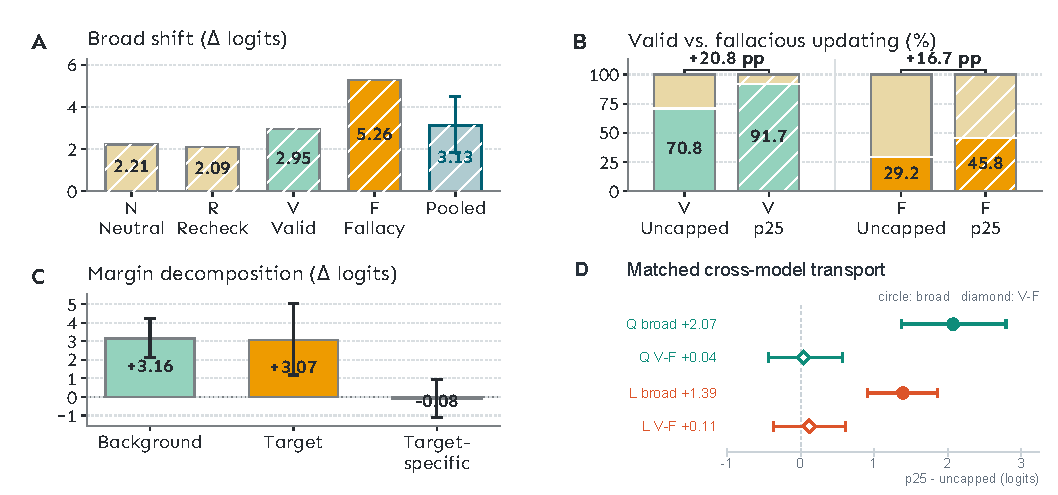
\includegraphics[width=\textwidth]{figures/cedar-figure2-results-v2-paper.pdf}
\caption{\textbf{Broad geometry shift and its categorical expression.} \textbf{(A--C)} Qwen development effects on broad margins, $V/F$ target following, and target-specificity. \textbf{(D)} Matched Qwen--Llama forced-choice transport. Whiskers are 95\% family-cluster bootstrap intervals; complete estimates appear in the appendix.}
\label{fig:behavioral-effects}
\end{figure*}

\subsection{Broad Compression of Initial-Answer Advantage}

The decomposition asks a direct question: did p25 make the proposed target more compelling, or did it make the current answer less dominant? In the exploratory Qwen bank, pooled $m_{\mathrm{general}}$ rose by $3.130$ logits (95\% CI $[1.834,4.486]$), while pooled target-specificity remained near zero (Figure~\ref{fig:behavioral-effects}A,C). Crucially, the broad shift also appeared in $N/R$, where the target was hidden; all corresponding choices nevertheless remained at $a_0$. When $V/F$ exposed the target, following rose by $20.8$ and $16.7$ points, leaving their difference essentially unchanged (Figure~\ref{fig:behavioral-effects}B). P25 therefore compressed initial-answer advantage broadly rather than selectively rewarding the valid warrant.
\subsection{A New Salt Retains the Geometric Direction and Changes the Transition Pattern}

The same-family new salt produced a complete-case increase of $1.538$ logits ($[0.455,2.741]$) in the average non-initial advantage over $a_0$. One planned continuous pair lacked logits, leaving the prespecified completeness rule unmet; worst-observed sensitivity retained the positive direction. The complete categorical ledger showed a different allocation: $V$ following fell by $12.5$ points while $F$ rose by $16.7$. Together with the complete matched-model assay, this sensitivity-supported recurrence makes broad displacement the common pattern across the tested same-family instances and released configurations, while categorical expression changes with task instantiation. Full sensitivity and scope details appear in Appendix Sections~E--F.

\subsection{Answer Geometry Moves Below the Choice Boundary}

The Social contrast shows the same separation from another angle. Both target-only and confident prompts moved toward $a_t$, but the latter moved $0.786$ logits less ($[-0.860,-0.711]$). In the fixed free-generation subset, no paired $S$ answer changed. Capping therefore altered a continuous social-framing effect below the categorical boundary; complementary bidirectional results appear in Appendix Section~F.
\subsection{Matched CEDAR-Evidence Transport Across Model-Specific Configurations}

Under matched forced choice, the broad shift was $+2.075$ logits for Qwen and $+1.391$ for Llama (Figure~\ref{fig:behavioral-effects}D). All arms moved in the same broad direction, while neither configuration showed a reliable continuous $V-F$ improvement. The pattern therefore transports to a second released model--axis pair under a common protocol; complete intervals, categorical changes, and configuration scope appear in Appendix Sections~D and F.

\section{Tracing the Hidden Displacement}
\label{sec:diagnosis}

Why does p25 capping move answer geometry without a stable gain in reason selectivity? We separate target exposure, intervention phase, an independent validity readout, trajectory composition, and visible-token changes, then follow the displacement beyond the capped layers.

\begin{figure*}[t]
\centering
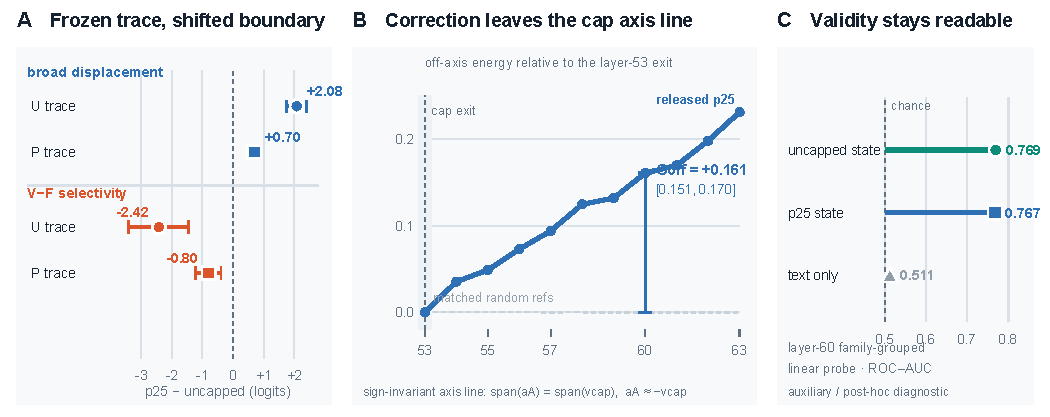
\includegraphics[width=\textwidth]{figures/cedar-figure3-mechanism-v2.pdf}
\caption{\textbf{Fixed-trace and representation diagnostics.} \textbf{(A)} The broad margin moves under token-identical replay. \textbf{(B)} The displacement composition rotates away from the cap's exit coordinate after rectification. \textbf{(C)} Layer-60 states retain condition-wise $V/F$ decodability. Intervals use the 12-family cluster bootstrap.}
\label{fig:mechanism-summary}
\end{figure*}

\subsection{The Shift Reappears in Either Phase}

Prefill-only and decode-only capping each reproduced nearly the full increase in mean $V/F$ target following: $+18.75$ and $+20.83$ points, versus $+18.75$ under full p25. The full effect was not their sum. The displacement is therefore accessible from either phase but is not explained by a simple additive split; complete intervals appear in Appendix Section~G.

\subsection{Revision Moves More Clearly than the Independent Validity Readout}

We measured warrant evaluation in an independent call that asked whether each $V/F$ reason was sufficient. Under full p25, common $V/F$ updating rose by $18.75$ points, whereas explicit validity discrimination had a $0.00$-point estimate with a family-cluster interval spanning substantial losses and gains. The point estimates do not move together, while the broad validity interval leaves preservation versus partial loss unresolved. This weak constraint motivates a downstream-use hypothesis without identifying the underlying mechanism.

\subsection{Trajectory Matching Resolves the Resistance-State Signal}

A development signal initially suggested that capping selectively hit a latent ``resistance state.'' Its prespecified test did not support that interpretation: resist-minus-yield correction was $-1.146$ $[-3.294,1.264]$, and the apparent exposure difference vanished after matching trajectory length ($0.033$ $[-1.394,2.166]$). Yield traces were roughly three times longer, revealing trajectory composition as the earlier confound. The result redirected the search from a special resistance moment to the answer decision itself.

\subsection{Answer Geometry Shifts under Token-Identical Replay}

The decisive test froze every visible reasoning token. We replayed uncapped- and p25-generated prefixes for 96 prompts through both forward conditions and read the answer logits. On uncapped-source traces, p25 still raised $m_{\mathrm{general}}$ by $2.078$ logits ($[1.759,2.408]$; Figure~\ref{fig:mechanism-summary}A), about two thirds of the natural-generation shift. P25-source traces also moved, though less. None of 192 paired replays crossed argmax: identical visible reasoning can therefore conceal a substantial change in the distribution from which the answer is selected. Continuous $V-F$ contrasts moved negatively under both trace sources, underscoring that the surviving shift was not a gain in reason selectivity. Replay definitions, interactions, and arm decompositions appear in Appendix Section~G.

\subsection{Downstream Displacement Rotates Away from the Exit Coordinate}

Finally, we asked how the fixed-trace displacement is composed after the capped window. Relative to the layer-53 exit direction, its off-axis energy share increased by $G_{\mathrm{off}}=0.161$ ($[0.151,0.170]$) by layer 60 (Figure~\ref{fig:mechanism-summary}B). All 12 families agreed in sign, whereas four schedule- and norm-matched random references showed almost no compositional change. A local one-axis correction is therefore remixed into a downstream state no longer summarized by its exit coordinate.

At that downstream layer, $V/F$ labels remained linearly decodable within each condition (ROC--AUC $0.769$ uncapped and $0.767$ capped), while a text-only baseline was near chance (Figure~\ref{fig:mechanism-summary}C). This establishes condition-wise decodability alongside downstream reorientation. Cross-condition transfer tests whether capped and uncapped states share a usable code; causal patching tests whether that signal participates in revision. Full layer curves, arm effects, controls, and probe protocol appear in Appendix Section~G.

Table~\ref{tab:diagnostic-chain} collects the chain: target concealment, an independent validity readout, trajectory matching, fixed-trace replay, and downstream reorientation progressively localize the broad displacement. Section~6 organizes this pattern as a testable mechanistic account.

\begin{table*}[t]
\centering
\small
\setlength{\tabcolsep}{4pt}
\renewcommand{\arraystretch}{1.12}
\begin{tabular}{@{}L{0.20\textwidth}L{0.38\textwidth}L{0.34\textwidth}@{}}
\toprule
Question tested & Decisive quantitative result & What the result reveals \\
\midrule

\textbf{Target-hidden}\newline
\textbf{movement}
&
With the target hidden, $\Delta m_{\mathrm{general}}$ remained positive in
$N/R$ ($+2.215/+2.092$ logits); pooled
$\Delta m_{\mathrm{specific}}=-0.084$ $[-1.110,0.953]$.
&
The shift does not require target exposure or target-specific attraction.
\\

\addlinespace

\textbf{Independent validity}\newline
\textbf{readout}
&
Under full p25, CommonUpdate increased by $18.75$ pp
$[4.17,33.33]$ while validity discrimination changed by $0.00$ pp;
layer-60 probe AUC was $0.769/0.767$.
&
The point estimates diverged; validity uncertainty leaves preservation versus partial loss unresolved.
\\

\addlinespace

\textbf{Token-identical}\newline
\textbf{replay}
&
On uncapped-source fixed traces, p25 increased
$m_{\mathrm{general}}$ by $2.078$ logits $[1.759,2.408]$; no visible token or
paired argmax changed.
&
The displacement survives token-identical reasoning below the choice boundary.
\\

\addlinespace

\textbf{Downstream}\newline
\textbf{composition}
&
After rectification stopped, off-exit-axis share increased by
$G_{\mathrm{off}}=0.161$ $[0.151,0.170]$; all 12 families were positive and
matched random references showed no comparable change.
&
The downstream displacement rotates away from its exit coordinate.
\\

\addlinespace

\textbf{Matched-model}\newline
\textbf{transport}
&
Under matched forced choice, $\Delta m_{\mathrm{general}}$ was
$+2.075$ $[1.372,2.791]$ for Qwen and $+1.391$ $[0.908,1.865]$ for Llama;
continuous $V-F$ changes stayed near zero.
&
The broad shift transports without a reliable selectivity gain.
\\

\bottomrule
\end{tabular}
\caption{\textbf{Diagnostic chain for the broad displacement.} Effects are p25 minus uncapped; intervals use the 12-family cluster bootstrap.}
\label{tab:diagnostic-chain}
\end{table*}

\section{Representational--Policy Decoupling as a Testable Account}
\label{sec:implications}

\subsection{The Hypothesis}

The diagnostic pattern motivates a separation between available information and its downstream use. The broad margin shift survives token-identical replay, the induced state-difference composition rotates off axis, and $V/F$ labels remain decodable within each condition. We call the resulting testable account \emph{representational--policy decoupling}: local rectification changes the state on which later layers operate and may thereby change the computation that maps reason-related structure and the current answer into option logits.

The hypothesis divides revision into two coupled objects. \emph{Representational content} includes the current answer, the proposed alternative, and structure indicating whether the offered warrant is valid. \emph{Revision policy} is the downstream mapping that propagates and weights those contents, compares the current answer with alternatives, and reads the result into option logits. Under ordinary inference, validity-sensitive structure can influence this mapping without appearing verbatim in the visible chain of thought.

P25 acts locally on a persona-related coordinate, and subsequent nonlinear layers operate on the rectified state. They can remix that correction into a multidimensional decision state, changing the relative support for the current answer even when the generated reasoning tokens remain fixed. Under the hypothesis, validity-related structure remains available while its downstream weighting changes. This account organizes the observed signature: target-hidden prompts move through current-answer geometry; $V$ and $F$ need not separate when the shift is not organized by warrant validity; different banks cross different choice boundaries; and the induced state difference leaves the coordinate on which it was imposed.

The hypothesis predicts a specific distinction. If the validity code itself is preserved, it should transfer across capped and uncapped states; if its downstream use is causal, restoring or protecting that route should recover reason selectivity without freezing all updates. Conversely, failure of cross-condition transfer would favor re-encoding or information loss over policy decoupling. These predictions turn the account into a mechanism program rather than a label for the present results.

\subsection{Toward Selective Control}

This account gives controller design two objectives: keep the model near a persona coordinate and preserve evidence-sensitive movement from representation to decision. One route separates \emph{detection} from \emph{actuation}: persona projection detects drift, while a redirected or gated correction protects components used to distinguish valid from invalid revision. Another is a two-stage controller that first evaluates the warrant and then modulates the strength or location of capping. Either design must be compared at matched persona benefit and must preserve valid updating while reducing fallacious and socially induced movement. A concrete protected-subspace ladder and its evaluation contract appear in Appendix Section~I.

\paragraph{Scope.}
The mapping-level evidence is strongest for the released Qwen p25 configuration; matched forced choice transports the broad shift, but not the mechanistic diagnostics, to the released Llama pair. New structural families, natural arguments, cross-condition probes, and activation patching are the direct tests of how broadly and causally the hypothesis holds.

\section{Conclusion}
\label{sec:conclusion}

CEDAR establishes a recurring answer-geometric effect of Assistant-Axis capping within its solver-certified family design and across two released model--axis configurations. Complete matched forced choice recovered the broad displacement in both configurations, with selectivity estimates centered near zero. Exploratory generation, target-hidden conditions, a same-family sensitivity analysis, and token-identical replay retained the geometric direction while categorical transitions varied. After rectification ended, the induced state-difference composition became more orthogonal to the cap's exit coordinate, and $V/F$ labels remained decodable within each condition.

Together, these results motivate representational--policy decoupling as a concrete mechanistic hypothesis: local rectification may alter the downstream mapping from reason-related state to revision. Cross-condition transfer and causal patching provide direct tests that distinguish shared-code preservation from re-encoding or information loss and probe the signal's causal role. CEDAR also separates two controller-evaluation objectives---persona stability and epistemically selective revision---and makes the second measurable.

% The aaai2027 package selects the required bibliography style automatically.
\bibliography{references}

\end{document}
